
\setcounter{section}{9}
\setcounter{subsection}{3}

\subsection{Linear Inequalities in Two Variables}

\begin{mdframed}
\textbf{Method:}
\begin{enumerate}
\item Replace the inequality symbol with an equal sign and graph the equation. Use a dashed line if the symbol is $<$ or $>$ and a solid line otherwise.
\item Decide on which side of the line to shade.
\begin{enumerate}
\item Choose a test point. If the inequality evaluated at the point is true, graph on the side that contains the test point; otherwise, graph the other side.
\item If the inequality is solved for $y$, shade based on the inequality symbol. Shade below the line if you have $y <\dots$ and shade above the line if you have $y > \dots$.
\end{enumerate}
\end{enumerate}
\end{mdframed}

\vspace{.3in}

\begin{example}
Graph: $4x - 2y \ge 8$
\begin{figure}[h]
\hfill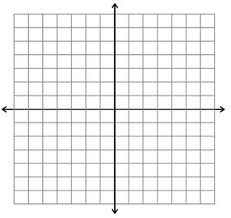
\includegraphics[scale=1.25]{images/plane}
\end{figure}
\vspace{1in}
\end{example}

\newpage

\begin{example}
Graph: $y > \dfrac{-3}{4}x$
\begin{figure}[h]
\hfill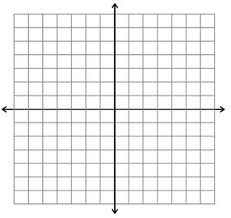
\includegraphics[scale=1.25]{images/plane}
\end{figure}
\vspace{1in}
\end{example}

\begin{example}
Graph: $x \le -2$
\begin{figure}[h]
\hfill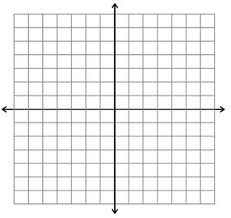
\includegraphics[scale=1.25]{images/plane}
\end{figure}
\vspace{1in}
\end{example}

\newpage

\begin{mdframed}
\textbf{Graphing Systems of Inequalities}

Systems of linear inequalities have a \emph{solution set} that is a portion of the plane, not just a point. To find this solution set, graph each of the inequalities individually and look for the overlap (intersection) of their solutions.
\end{mdframed}
\vspace{.2in}

\begin{example}
Graph the solution set of the following system:
\begin{align*}[left=\empheqlbrace]
x-3y&<6\\
 2x+3y&\ge -6
 \end{align*}
\begin{figure}[h]
\hfill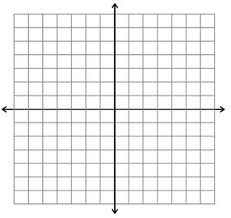
\includegraphics[scale=1.25]{images/plane}
\end{figure}
\vspace{1in}
\end{example}

\newpage

\begin{example}
Graph the solution set of the following system:
\begin{align*}[left=\empheqlbrace]
x+y&<2\\
-2\le x &< 1\\
 y &> -3
 \end{align*}
\begin{figure}[h]
\hfill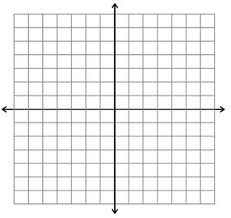
\includegraphics[scale=1.25]{images/plane}
\end{figure}
\vspace{1in}
\end{example}